\documentclass[aspectratio=169]{beamer}

\usetheme{default}
\usecolortheme{dove}

\setbeamertemplate{navigation symbols}{}
\setbeamertemplate{footline}{%
  \hfill\insertframenumber\,/\,\inserttotalframenumber\hspace{0.5em}\vspace{0.5em}%
}

\definecolor{popblue}{RGB}{52, 101, 164}
\definecolor{sampred}{RGB}{204, 0, 0}
\definecolor{paramgreen}{RGB}{0, 140, 70}
\definecolor{warnred}{RGB}{180, 40, 40}
\definecolor{orange1}{RGB}{220, 120, 0}

\setbeamercolor{frametitle}{fg=popblue}
\setbeamercolor{title}{fg=popblue}

\usepackage{pgfplots}
\usepackage{tikz}
\usetikzlibrary{shapes, arrows.meta, positioning, calc, decorations.pathreplacing, patterns}
\pgfplotsset{compat=1.18}
\usepackage{amsmath, amssymb}

\title{Lecture 1: Descriptive Statistics}
\subtitle{and Empirical Distributions}
\date{}

\begin{document}

% ============================================================
\begin{frame}
\titlepage
\end{frame}

% ============================================================
\begin{frame}
\frametitle{You get a spreadsheet with 10,000 rows\ldots}
\begin{center}
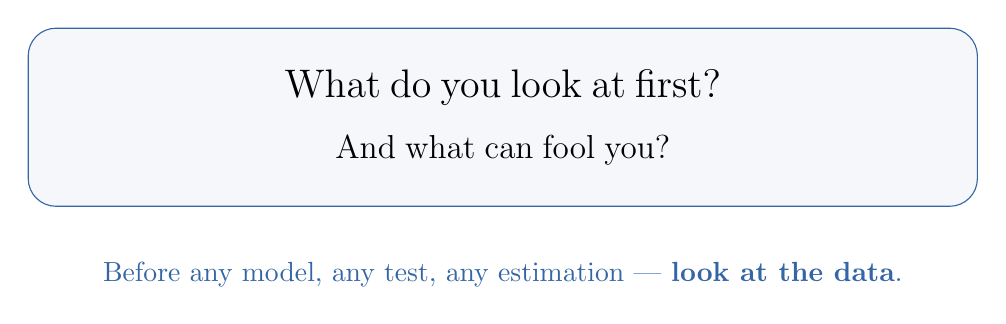
\begin{tikzpicture}
  \node[draw=popblue, fill=popblue!5, rounded corners=10pt, text width=11cm, align=center, inner sep=15pt] {
    {\Large What do you look at first?}\\[10pt]
    {\large And what can fool you?}
  };
  \node[font=\normalsize, text=popblue] at (0, -2) {Before any model, any test, any estimation --- \textbf{look at the data}.};
\end{tikzpicture}
\end{center}
\end{frame}

% ============================================================
\begin{frame}
\frametitle{Goals of Descriptive Statistics}
\begin{center}
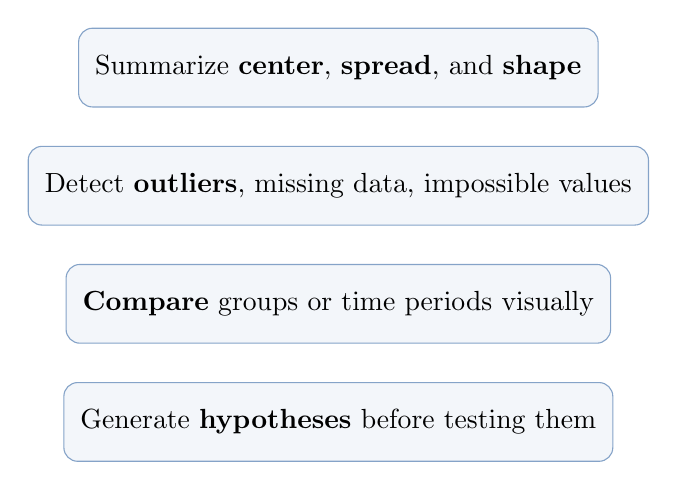
\begin{tikzpicture}[
  gbox/.style={draw=popblue!60, fill=popblue!6, rounded corners=5pt, minimum width=5cm, minimum height=1cm, align=center, font=\normalsize, inner sep=6pt}
]
  \node[gbox] at (0, 2.5) {Summarize \textbf{center}, \textbf{spread}, and \textbf{shape}};
  \node[gbox] at (0, 1) {Detect \textbf{outliers}, missing data, impossible values};
  \node[gbox] at (0, -0.5) {\textbf{Compare} groups or time periods visually};
  \node[gbox] at (0, -2) {Generate \textbf{hypotheses} before testing them};
\end{tikzpicture}
\end{center}
\vspace{0.4cm}
\begin{center}
\small Descriptive $\ne$ inferential: we're describing \textit{this sample}, not yet the population.
\end{center}
\end{frame}

% ============================================================
\section{Measures of Center}

\begin{frame}
\frametitle{Measures of Center}
\begin{center}
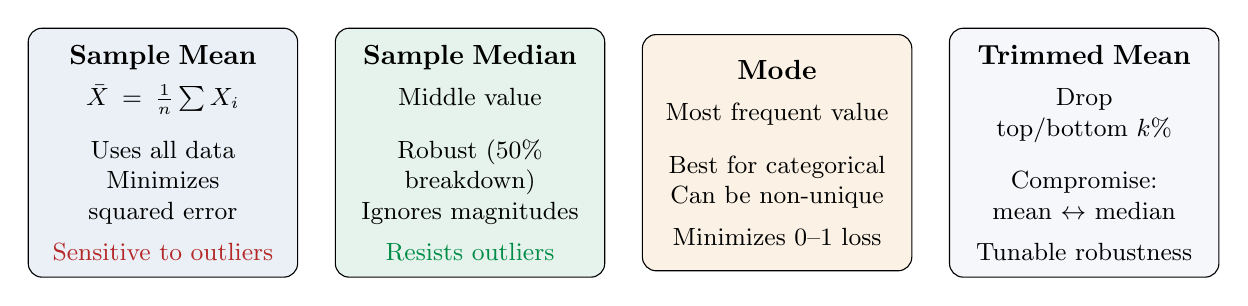
\begin{tikzpicture}[
  mbox/.style={draw, rounded corners=5pt, minimum width=3.2cm, minimum height=3cm, align=center, text width=3cm, inner sep=6pt, font=\small}
]
  \node[mbox, fill=popblue!10] at (-5.2, 0) {
    \textbf{\normalsize Sample Mean}\\[4pt]
    $\bar{X} = \frac{1}{n}\sum X_i$\\[8pt]
    Uses all data\\
    Minimizes squared error\\[4pt]
    \textcolor{warnred}{Sensitive to outliers}
  };
  \node[mbox, fill=paramgreen!10] at (-1.3, 0) {
    \textbf{\normalsize Sample Median}\\[4pt]
    Middle value\\[8pt]
    Robust (50\% breakdown)\\
    Ignores magnitudes\\[4pt]
    \textcolor{paramgreen}{Resists outliers}
  };
  \node[mbox, fill=orange1!10] at (2.6, 0) {
    \textbf{\normalsize Mode}\\[4pt]
    Most frequent value\\[8pt]
    Best for categorical\\
    Can be non-unique\\[4pt]
    Minimizes 0--1 loss
  };
  \node[mbox, fill=popblue!5] at (6.5, 0) {
    \textbf{\normalsize Trimmed Mean}\\[4pt]
    Drop top/bottom $k\%$\\[8pt]
    Compromise:\\
    mean $\leftrightarrow$ median\\[4pt]
    Tunable robustness
  };
\end{tikzpicture}
\end{center}
\end{frame}

\begin{frame}
\frametitle{The Billionaire in the Room}
\begin{center}
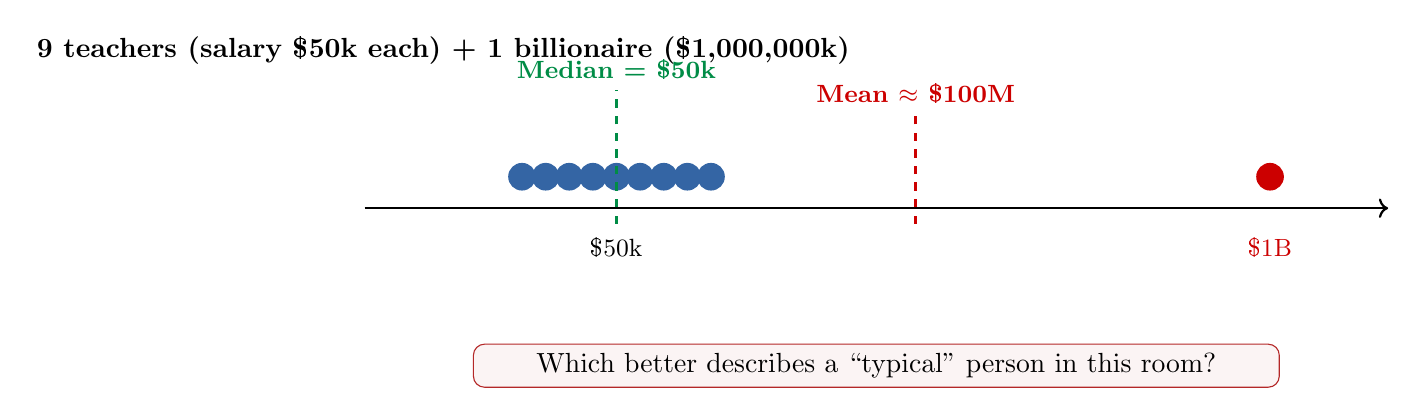
\begin{tikzpicture}
  % People icons as dots
  \node[font=\bfseries] at (0, 3.5) {9 teachers (salary \$50k each) + 1 billionaire (\$1{,}000{,}000k)};

  % Dot plot
  \draw[thick, ->] (-1, 1.5) -- (12, 1.5);

  % Teacher dots clustered at 50k
  \foreach \i in {0,...,8} {
    \fill[popblue] (1 + 0.3*\i, 1.9) circle (5pt);
  }
  \node[font=\small] at (2.2, 1.0) {\$50k};

  % Billionaire dot far right
  \fill[sampred] (10.5, 1.9) circle (5pt);
  \node[font=\small, sampred] at (10.5, 1.0) {\$1B};

  % Mean
  \draw[very thick, sampred, dashed] (6, 1.3) -- (6, 2.7);
  \node[font=\small\bfseries, sampred, above] at (6, 2.7) {Mean $\approx$ \$100M};

  % Median
  \draw[very thick, paramgreen, dashed] (2.2, 1.3) -- (2.2, 3.0);
  \node[font=\small\bfseries, paramgreen, above] at (2.2, 3.0) {Median = \$50k};

  % Verdict
  \node[draw=warnred, fill=warnred!5, rounded corners=4pt, font=\normalsize, text width=10cm, align=center] at (5.5, -0.5) {
    Which better describes a ``typical'' person in this room?
  };
\end{tikzpicture}
\end{center}
\end{frame}

% ============================================================
\section{Measures of Spread}

\begin{frame}
\frametitle{Measures of Spread}
\begin{center}
\renewcommand{\arraystretch}{1.6}
\begin{tabular}{lcp{5.5cm}}
  \textbf{Measure} & \textbf{Formula} & \textbf{Properties} \\
  \hline
  Variance $S^2$ & $\frac{1}{n-1}\sum(X_i - \bar{X})^2$ & Uses all data; $n{-}1$ = Bessel's correction (unbiased) \\
  Std Dev $S$ & $\sqrt{S^2}$ & Same units as data \\
  Range & $\max - \min$ & Simple; extremely fragile \\
  IQR & $Q_3 - Q_1$ & Middle 50\%; robust \\
  MAD & $\text{med}\,|X_i - \text{med}|$ & Most robust; companion to median \\
  CV & $S / \bar{X}$ & Dimensionless; compare across scales \\
  \hline
\end{tabular}
\end{center}

\vspace{0.3cm}
\begin{center}
\small \textbf{Why $n-1$?} We used up one ``degree of freedom'' estimating $\bar{X}$.\\
(We'll prove $\mathbb{E}[S^2] = \sigma^2$ in Lecture 3.)
\end{center}
\end{frame}

\begin{frame}
\frametitle{Robust vs Non-Robust: Visual}
\begin{center}
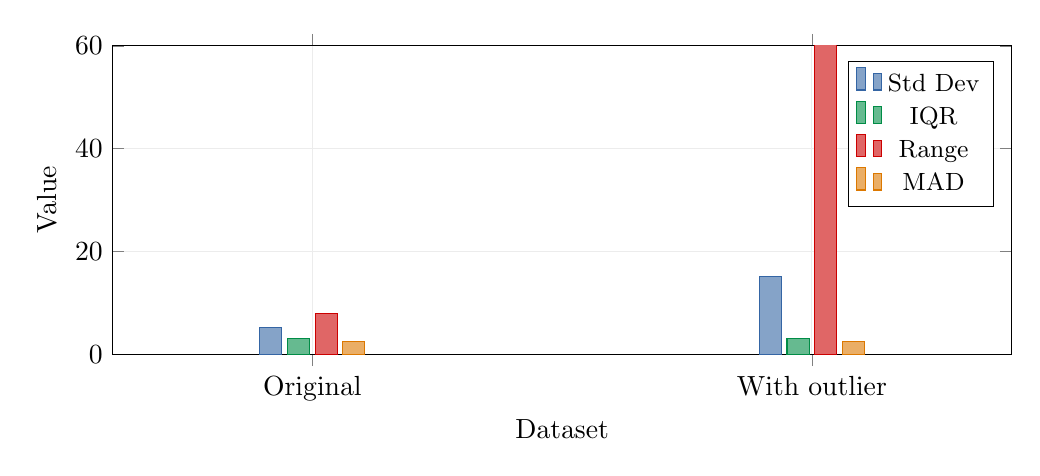
\begin{tikzpicture}
  \begin{axis}[
    width=13cm, height=5.5cm,
    ybar, bar width=8pt,
    xlabel={Dataset},
    ylabel={Value},
    xtick={1,2},
    xticklabels={Original, With outlier},
    ymin=0, ymax=60,
    legend style={at={(0.98,0.95)}, anchor=north east, font=\small},
    grid=major, grid style={gray!15},
    enlarge x limits=0.4,
  ]
    % Original
    \addplot[fill=popblue!60, draw=popblue] coordinates {(1, 5.2) (2, 15.1)};
    \addlegendentry{Std Dev}
    \addplot[fill=paramgreen!60, draw=paramgreen] coordinates {(1, 3.0) (2, 3.0)};
    \addlegendentry{IQR}
    \addplot[fill=sampred!60, draw=sampred] coordinates {(1, 8) (2, 95)};
    \addlegendentry{Range}
    \addplot[fill=orange1!60, draw=orange1] coordinates {(1, 2.5) (2, 2.5)};
    \addlegendentry{MAD}
  \end{axis}
\end{tikzpicture}
\end{center}
\vspace{0.1cm}
\begin{center}
\small One outlier: Range explodes, Std Dev triples. IQR and MAD don't budge.
\end{center}
\end{frame}

% ============================================================
\section{Quantiles and Boxplots}

\begin{frame}
\frametitle{Quantiles and Percentiles}
\begin{center}
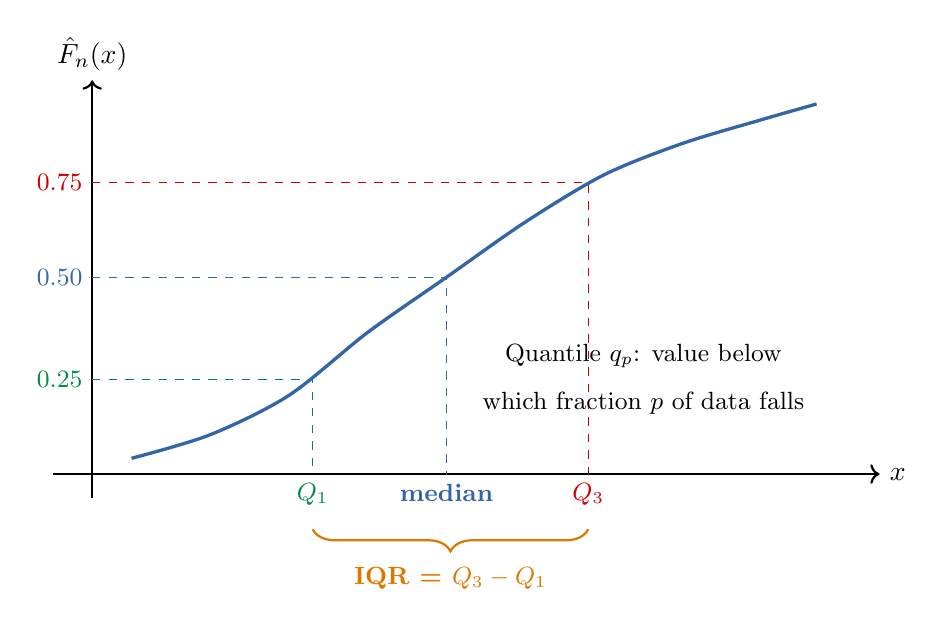
\begin{tikzpicture}
  % CDF-like curve
  \draw[thick, ->] (-0.5, 0) -- (10, 0) node[right] {$x$};
  \draw[thick, ->] (0, -0.3) -- (0, 5) node[above] {$\hat{F}_n(x)$};

  % S-curve
  \draw[very thick, popblue, smooth] plot coordinates {
    (0.5, 0.2) (1.5, 0.5) (2.5, 1.0) (3.5, 1.8) (4.5, 2.5)
    (5.5, 3.2) (6.5, 3.8) (7.5, 4.2) (8.5, 4.5) (9.2, 4.7)
  };

  % Horizontal lines at 25%, 50%, 75%
  \draw[dashed, paramgreen] (0, 1.2) -- (2.8, 1.2) -- (2.8, 0);
  \node[left, font=\small, paramgreen] at (0, 1.2) {0.25};
  \node[below, font=\small\bfseries, paramgreen] at (2.8, 0) {$Q_1$};

  \draw[dashed, popblue] (0, 2.5) -- (4.5, 2.5) -- (4.5, 0);
  \node[left, font=\small, popblue] at (0, 2.5) {0.50};
  \node[below, font=\small\bfseries, popblue] at (4.5, 0) {median};

  \draw[dashed, sampred] (0, 3.7) -- (6.3, 3.7) -- (6.3, 0);
  \node[left, font=\small, sampred] at (0, 3.7) {0.75};
  \node[below, font=\small\bfseries, sampred] at (6.3, 0) {$Q_3$};

  % IQR brace
  \draw[decorate, decoration={brace, amplitude=8pt, mirror}, thick, orange1]
    (2.8, -0.7) -- (6.3, -0.7) node[midway, below=10pt, font=\small\bfseries, orange1] {IQR = $Q_3 - Q_1$};

  % Labels
  \node[font=\small] at (7, 1.5) {Quantile $q_p$: value below};
  \node[font=\small] at (7, 0.9) {which fraction $p$ of data falls};
\end{tikzpicture}
\end{center}
\end{frame}

\begin{frame}
\frametitle{Boxplot Anatomy}
\begin{center}
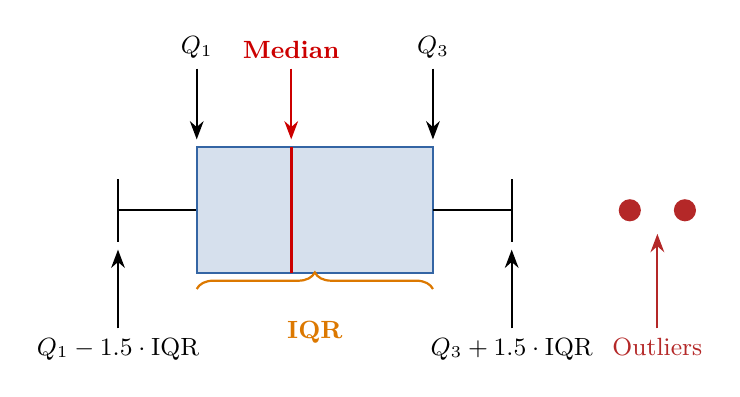
\begin{tikzpicture}
  % The boxplot (horizontal)
  \draw[thick] (2, 0) -- (7, 0); % lower whisker
  \draw[thick] (2, -0.4) -- (2, 0.4); % lower whisker cap
  \fill[popblue!20, draw=popblue, thick] (3, -0.8) rectangle (6, 0.8); % box
  \draw[very thick, sampred] (4.2, -0.8) -- (4.2, 0.8); % median
  \draw[thick] (7, -0.4) -- (7, 0.4); % upper whisker cap
  \draw[thick] (6, 0) -- (7, 0); % upper whisker

  % Outlier dots
  \fill[warnred] (8.5, 0) circle (4pt);
  \fill[warnred] (9.2, 0) circle (4pt);

  % Labels with arrows
  \draw[-{Stealth}, thick] (2, -1.5) -- (2, -0.5);
  \node[font=\small, below] at (2, -1.5) {$Q_1 - 1.5 \cdot\text{IQR}$};

  \draw[-{Stealth}, thick] (3, 1.8) -- (3, 0.9);
  \node[font=\small, above] at (3, 1.8) {$Q_1$};

  \draw[-{Stealth}, thick, sampred] (4.2, 1.8) -- (4.2, 0.9);
  \node[font=\small\bfseries, above, sampred] at (4.2, 1.8) {Median};

  \draw[-{Stealth}, thick] (6, 1.8) -- (6, 0.9);
  \node[font=\small, above] at (6, 1.8) {$Q_3$};

  \draw[-{Stealth}, thick] (7, -1.5) -- (7, -0.5);
  \node[font=\small, below] at (7, -1.5) {$Q_3 + 1.5 \cdot\text{IQR}$};

  \draw[-{Stealth}, thick, warnred] (8.85, -1.5) -- (8.85, -0.3);
  \node[font=\small, below, warnred] at (8.85, -1.5) {Outliers};

  % IQR brace
  \draw[decorate, decoration={brace, amplitude=6pt}, thick, orange1]
    (3, -1.0) -- (6, -1.0) node[midway, below=8pt, font=\small\bfseries, orange1] {IQR};
\end{tikzpicture}
\end{center}

\vspace{0.5cm}
\begin{columns}
\begin{column}{0.48\textwidth}
\textbf{Strengths:}
\begin{itemize}
  \small
  \item Compact group comparison
  \item Shows center, spread, outliers
\end{itemize}
\end{column}
\begin{column}{0.48\textwidth}
\textbf{Weakness:}
\begin{itemize}
  \small
  \item Hides multimodality!
  \item Pair with histogram or violin
\end{itemize}
\end{column}
\end{columns}
\end{frame}

\begin{frame}
\frametitle{Boxplot Hides Bimodality}
\begin{center}
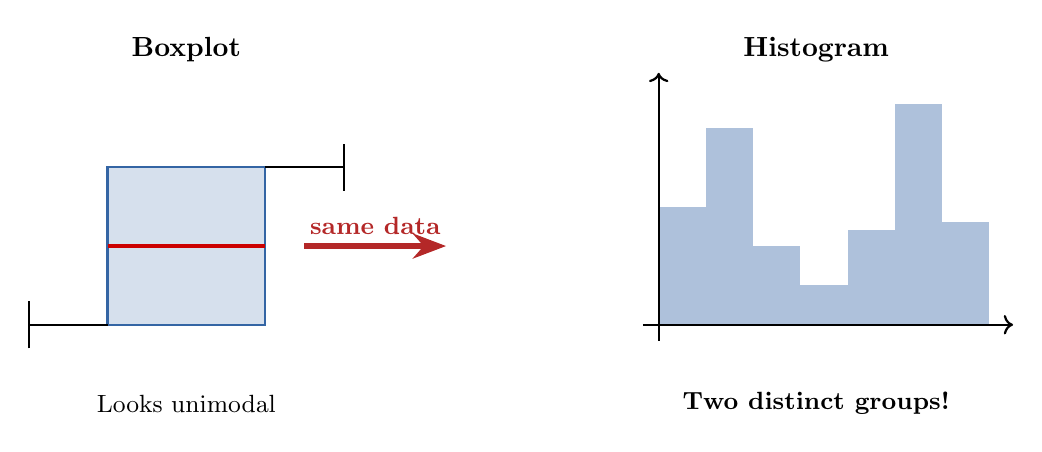
\begin{tikzpicture}
  % Left: the boxplot
  \begin{scope}[xshift=-4cm]
    \node[font=\bfseries] at (2, 3.5) {Boxplot};
    \fill[popblue!20, draw=popblue, thick] (1, 0) rectangle (3, 2);
    \draw[very thick, sampred] (1, 1) -- (3, 1);
    \draw[thick] (0, 0) -- (1, 0); \draw[thick] (0, -0.3) -- (0, 0.3);
    \draw[thick] (3, 2) -- (4, 2); \draw[thick] (4, 1.7) -- (4, 2.3);
    \node[font=\small] at (2, -1) {Looks unimodal};
  \end{scope}

  % Right: the histogram (bimodal)
  \begin{scope}[xshift=4cm]
    \node[font=\bfseries] at (2, 3.5) {Histogram};
    \fill[popblue!40] (0, 0) rectangle (0.6, 1.5);
    \fill[popblue!40] (0.6, 0) rectangle (1.2, 2.5);
    \fill[popblue!40] (1.2, 0) rectangle (1.8, 1.0);
    \fill[popblue!40] (1.8, 0) rectangle (2.4, 0.5);
    \fill[popblue!40] (2.4, 0) rectangle (3.0, 1.2);
    \fill[popblue!40] (3.0, 0) rectangle (3.6, 2.8);
    \fill[popblue!40] (3.6, 0) rectangle (4.2, 1.3);
    \draw[thick, ->] (-0.2, 0) -- (4.5, 0);
    \draw[thick, ->] (0, -0.2) -- (0, 3.2);
    \node[font=\small] at (2, -1) {\textbf{Two distinct groups!}};
  \end{scope}

  % Arrow
  \draw[-{Stealth}, very thick, warnred, line width=2pt] (-0.5, 1) -- (1.3, 1)
    node[midway, above, font=\small\bfseries, warnred] {same data};
\end{tikzpicture}
\end{center}

\vspace{0.3cm}
\begin{center}
\fcolorbox{warnred}{warnred!5}{\parbox{10cm}{\centering\small Always pair boxplots with histograms or violin plots.}}
\end{center}
\end{frame}

\begin{frame}
\frametitle{Quantiles in the Real World}
\begin{center}
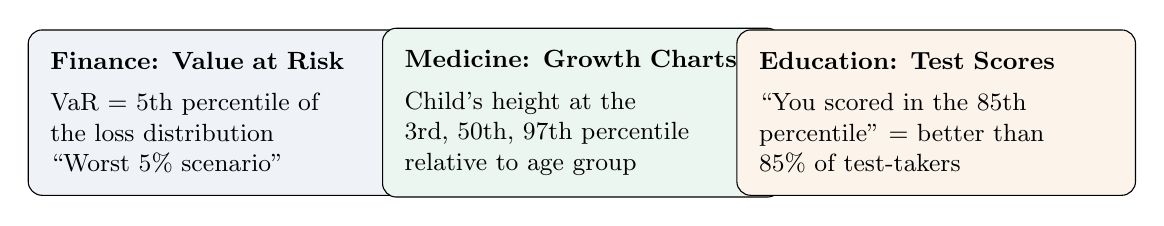
\begin{tikzpicture}[
  appbox/.style={draw, rounded corners=5pt, minimum height=1.8cm, text width=4.5cm, align=left, inner sep=8pt, font=\small}
]
  \node[appbox, fill=popblue!8] at (-4.5, 0) {
    \textbf{Finance: Value at Risk}\\[4pt]
    VaR = 5th percentile of\\
    the loss distribution\\
    ``Worst 5\% scenario''
  };
  \node[appbox, fill=paramgreen!8] at (0, 0) {
    \textbf{Medicine: Growth Charts}\\[4pt]
    Child's height at the\\
    3rd, 50th, 97th percentile\\
    relative to age group
  };
  \node[appbox, fill=orange1!8] at (4.5, 0) {
    \textbf{Education: Test Scores}\\[4pt]
    ``You scored in the 85th\\
    percentile'' = better than\\
    85\% of test-takers
  };
\end{tikzpicture}
\end{center}
\end{frame}

% ============================================================
\section{Shape: Skewness and Kurtosis}

\begin{frame}
\frametitle{Skewness: Measuring Asymmetry}
\begin{center}
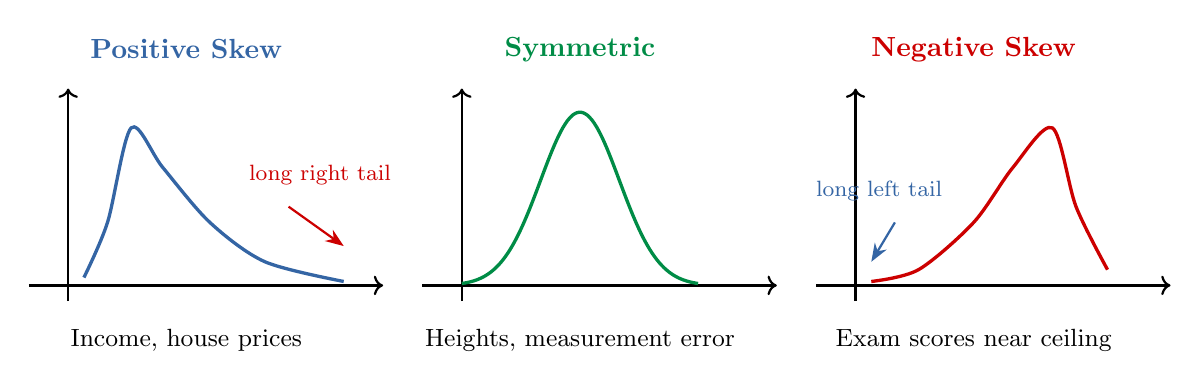
\begin{tikzpicture}
  % Positive skew
  \begin{scope}[xshift=-5cm]
    \node[font=\bfseries, popblue] at (1.5, 3) {Positive Skew};
    \draw[thick, ->] (-0.5, 0) -- (4, 0);
    \draw[thick, ->] (0, -0.2) -- (0, 2.5);
    \draw[very thick, popblue, smooth] plot coordinates {
      (0.2, 0.1) (0.5, 0.8) (0.8, 2.0) (1.2, 1.5) (1.8, 0.8) (2.5, 0.3) (3.5, 0.05)
    };
    \node[font=\small] at (1.5, -0.7) {Income, house prices};
    \draw[-{Stealth}, thick, sampred] (2.8, 1) -- (3.5, 0.5);
    \node[font=\footnotesize, sampred] at (3.2, 1.4) {long right tail};
  \end{scope}

  % Symmetric
  \begin{scope}[xshift=0cm]
    \node[font=\bfseries, paramgreen] at (1.5, 3) {Symmetric};
    \draw[thick, ->] (-0.5, 0) -- (4, 0);
    \draw[thick, ->] (0, -0.2) -- (0, 2.5);
    \draw[very thick, paramgreen, smooth, domain=0:3, samples=50] plot (\x, {2.2*exp(-(\x-1.5)*(\x-1.5)/0.5)});
    \node[font=\small] at (1.5, -0.7) {Heights, measurement error};
  \end{scope}

  % Negative skew
  \begin{scope}[xshift=5cm]
    \node[font=\bfseries, sampred] at (1.5, 3) {Negative Skew};
    \draw[thick, ->] (-0.5, 0) -- (4, 0);
    \draw[thick, ->] (0, -0.2) -- (0, 2.5);
    \draw[very thick, sampred, smooth] plot coordinates {
      (0.2, 0.05) (0.8, 0.2) (1.5, 0.8) (2.0, 1.5) (2.5, 2.0) (2.8, 1.0) (3.2, 0.2)
    };
    \node[font=\small] at (1.5, -0.7) {Exam scores near ceiling};
    \draw[-{Stealth}, thick, popblue] (0.5, 0.8) -- (0.2, 0.3);
    \node[font=\footnotesize, popblue] at (0.3, 1.2) {long left tail};
  \end{scope}
\end{tikzpicture}
\end{center}

\vspace{0.2cm}
$$\text{Skewness} = \frac{1}{n}\sum_{i=1}^n\left(\frac{X_i - \bar{X}}{S}\right)^3$$
\end{frame}

\begin{frame}
\frametitle{Kurtosis: Tail Heaviness}
\begin{center}
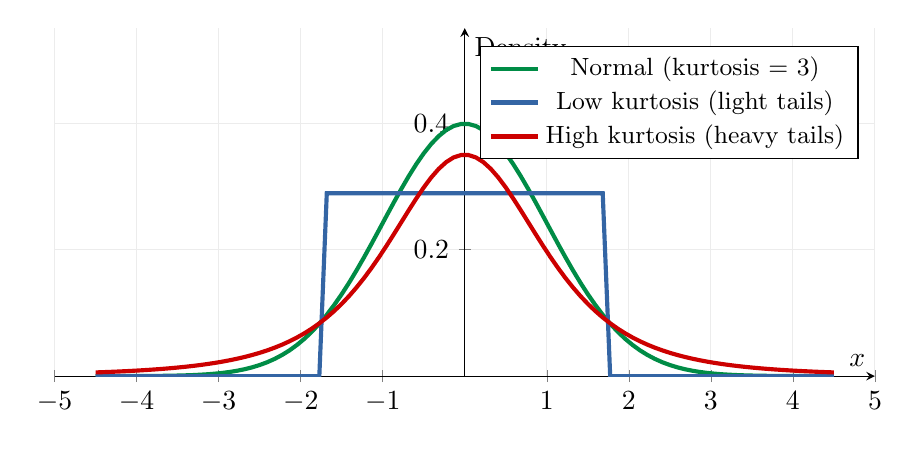
\begin{tikzpicture}
  \begin{axis}[
    width=12cm, height=6cm,
    xlabel={$x$},
    ylabel={Density},
    xmin=-5, xmax=5,
    ymin=0, ymax=0.55,
    axis lines=middle,
    legend style={at={(0.98,0.95)}, anchor=north east, font=\small},
    grid=major, grid style={gray!15},
    every axis plot/.append style={line width=1.5pt, samples=100}
  ]
    % Normal (kurtosis = 3)
    \addplot[paramgreen, domain=-4.5:4.5] {exp(-x^2/2) / sqrt(2*pi)};
    \addlegendentry{Normal (kurtosis = 3)}

    % Low kurtosis (uniform-ish)
    \addplot[popblue, domain=-4.5:4.5] {(abs(x) < 1.73) * 0.289};
    \addlegendentry{Low kurtosis (light tails)}

    % High kurtosis (t-distribution like)
    \addplot[sampred, domain=-4.5:4.5] {0.35 / (1 + x^2/3)^2};
    \addlegendentry{High kurtosis (heavy tails)}
  \end{axis}
\end{tikzpicture}
\end{center}
\vspace{0.1cm}
\begin{center}
\small High kurtosis $\Rightarrow$ more extreme outliers than normal predicts.\\
\small Financial returns have high kurtosis --- assuming normality underestimates risk.
\end{center}
\end{frame}

% ============================================================
\section{The Empirical CDF}

\begin{frame}
\frametitle{The Empirical CDF}

$$\hat{F}_n(t) = \frac{1}{n}\#\{X_i \le t\} = \frac{\text{number of observations} \le t}{n}$$

\begin{center}
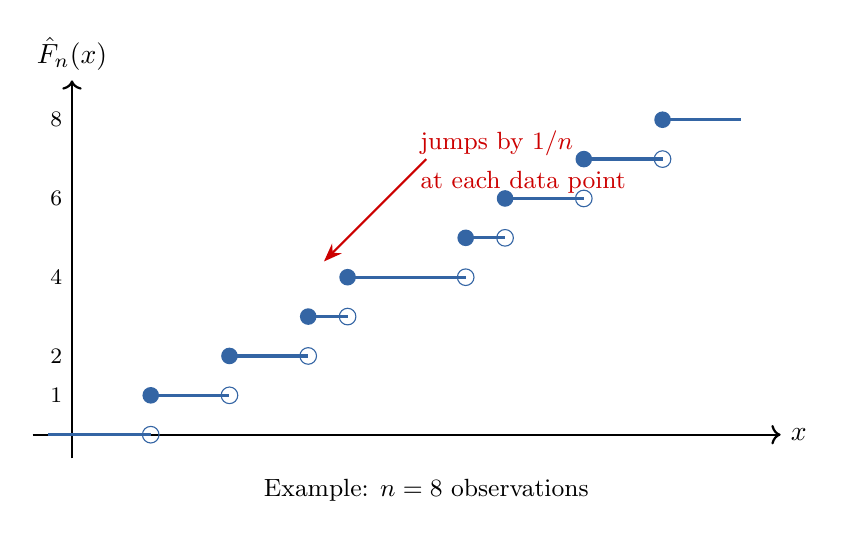
\begin{tikzpicture}
  \draw[thick, ->] (-0.5, 0) -- (9, 0) node[right] {$x$};
  \draw[thick, ->] (0, -0.3) -- (0, 4.5) node[above] {$\hat{F}_n(x)$};

  % Step function (n=8 example)
  \draw[very thick, popblue]
    (-0.3, 0) -- (1, 0)
    (1, 0.5) -- (2, 0.5)
    (2, 1.0) -- (3, 1.0)
    (3, 1.5) -- (3.5, 1.5)
    (3.5, 2.0) -- (5, 2.0)
    (5, 2.5) -- (5.5, 2.5)
    (5.5, 3.0) -- (6.5, 3.0)
    (6.5, 3.5) -- (7.5, 3.5)
    (7.5, 4.0) -- (8.5, 4.0);

  % Jump dots
  \foreach \x/\y in {1/0.5, 2/1.0, 3/1.5, 3.5/2.0, 5/2.5, 5.5/3.0, 6.5/3.5, 7.5/4.0} {
    \fill[popblue] (\x, \y) circle (3pt);
    \draw[popblue] (\x, \y-0.5) circle (3pt);
  }

  % Y-axis labels
  \foreach \y/\lab in {0.5/1/8, 1.0/2/8, 2.0/4/8, 3.0/6/8, 4.0/8/8} {
    \node[left, font=\footnotesize] at (0, \y) {$\lab$};
  }

  % Annotation
  \draw[-{Stealth}, thick, sampred] (4.5, 3.5) -- (3.2, 2.2);
  \node[font=\small, sampred, right] at (4.3, 3.7) {jumps by $1/n$};
  \node[font=\small, sampred, right] at (4.3, 3.2) {at each data point};

  % n label
  \node[font=\small] at (4.5, -0.7) {Example: $n = 8$ observations};
\end{tikzpicture}
\end{center}
\end{frame}

\begin{frame}
\frametitle{ECDF: Why It's Powerful}
\begin{center}
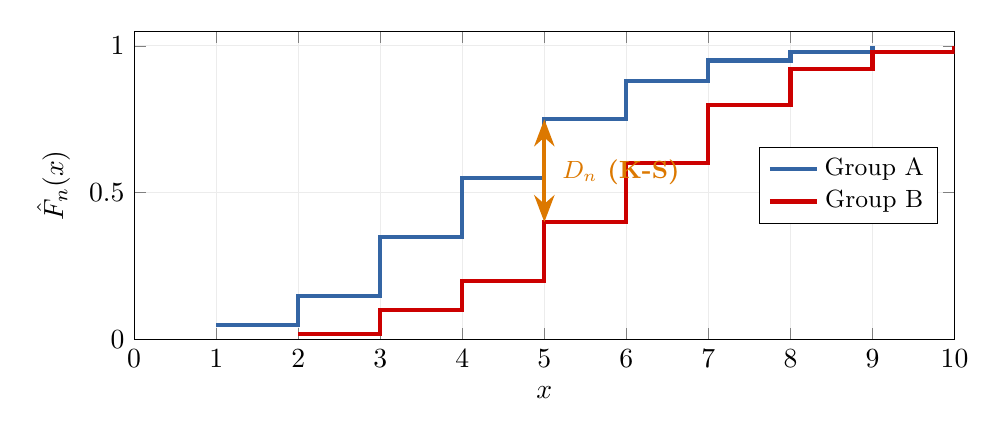
\begin{tikzpicture}
  \begin{axis}[
    width=12cm, height=5.5cm,
    xlabel={$x$},
    ylabel={$\hat{F}_n(x)$},
    xmin=0, xmax=10,
    ymin=0, ymax=1.05,
    legend style={at={(0.98,0.5)}, anchor=east, font=\small},
    grid=major, grid style={gray!15},
    every axis plot/.append style={line width=1.5pt}
  ]
    % Group A ECDF
    \addplot[popblue, const plot] coordinates {
      (1, 0.05) (2, 0.15) (3, 0.35) (4, 0.55) (5, 0.75) (6, 0.88) (7, 0.95) (8, 0.98) (9, 1.0)
    };
    \addlegendentry{Group A}

    % Group B ECDF (shifted right)
    \addplot[sampred, const plot] coordinates {
      (2, 0.02) (3, 0.10) (4, 0.20) (5, 0.40) (6, 0.60) (7, 0.80) (8, 0.92) (9, 0.98) (10, 1.0)
    };
    \addlegendentry{Group B}

    % KS distance
    \draw[{Stealth}-{Stealth}, thick, orange1, line width=1.5pt] (axis cs:5, 0.40) -- (axis cs:5, 0.75);
    \node[font=\small\bfseries, orange1, right] at (axis cs:5.1, 0.57) {$D_n$ (K-S)};
  \end{axis}
\end{tikzpicture}
\end{center}

\begin{itemize}
  \small
  \item No bin-width choice (unlike histograms) --- the ECDF is \textbf{parameter-free}
  \item Biggest gap = \textbf{Kolmogorov--Smirnov statistic} (formalized in Lecture 7)
  \item Glivenko--Cantelli: $\hat{F}_n \to F$ uniformly as $n \to \infty$
\end{itemize}
\end{frame}

% ============================================================
\section{Summary Statistics Can Lie}

\begin{frame}
\frametitle{Anscombe's Quartet (1973)}
\begin{center}
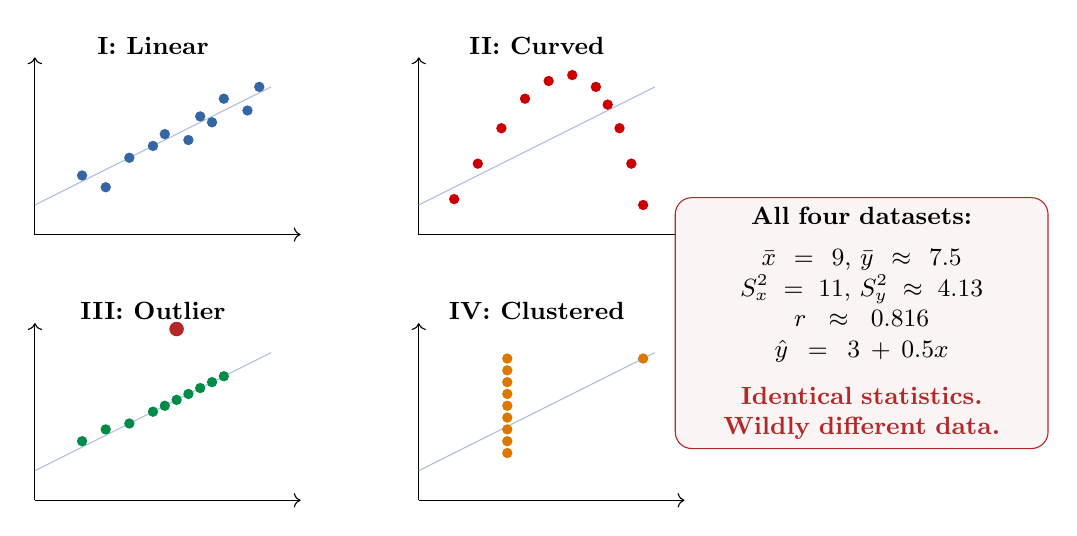
\begin{tikzpicture}[scale=0.75]
  % All four have same: mean x=9, mean y=7.5, var x=11, var y=4.13, corr=0.816, regression: y=3+0.5x

  % Dataset I - linear
  \begin{scope}[xshift=-5.5cm, yshift=2.5cm]
    \node[font=\small\bfseries] at (2, 3.2) {I: Linear};
    \draw[->] (0,0) -- (4.5, 0); \draw[->] (0,0) -- (0, 3);
    \draw[thin, popblue!40] (0, 0.5) -- (4, 2.5);
    \foreach \x/\y in {0.8/1.0, 1.2/0.8, 1.6/1.3, 2.0/1.5, 2.2/1.7, 2.6/1.6, 2.8/2.0, 3.0/1.9, 3.2/2.3, 3.6/2.1, 3.8/2.5} {
      \fill[popblue] (\x, \y) circle (2.5pt);
    }
  \end{scope}

  % Dataset II - curved
  \begin{scope}[xshift=1cm, yshift=2.5cm]
    \node[font=\small\bfseries] at (2, 3.2) {II: Curved};
    \draw[->] (0,0) -- (4.5, 0); \draw[->] (0,0) -- (0, 3);
    \draw[thin, popblue!40] (0, 0.5) -- (4, 2.5);
    \foreach \x/\y in {0.6/0.6, 1.0/1.2, 1.4/1.8, 1.8/2.3, 2.2/2.6, 2.6/2.7, 3.0/2.5, 3.2/2.2, 3.4/1.8, 3.6/1.2, 3.8/0.5} {
      \fill[sampred] (\x, \y) circle (2.5pt);
    }
  \end{scope}

  % Dataset III - outlier
  \begin{scope}[xshift=-5.5cm, yshift=-2cm]
    \node[font=\small\bfseries] at (2, 3.2) {III: Outlier};
    \draw[->] (0,0) -- (4.5, 0); \draw[->] (0,0) -- (0, 3);
    \draw[thin, popblue!40] (0, 0.5) -- (4, 2.5);
    \foreach \x/\y in {0.8/1.0, 1.2/1.2, 1.6/1.3, 2.0/1.5, 2.2/1.6, 2.4/1.7, 2.6/1.8, 2.8/1.9, 3.0/2.0, 3.2/2.1} {
      \fill[paramgreen] (\x, \y) circle (2.5pt);
    }
    \fill[warnred] (2.4, 2.9) circle (3.5pt); % outlier
  \end{scope}

  % Dataset IV - clustered + extreme
  \begin{scope}[xshift=1cm, yshift=-2cm]
    \node[font=\small\bfseries] at (2, 3.2) {IV: Clustered};
    \draw[->] (0,0) -- (4.5, 0); \draw[->] (0,0) -- (0, 3);
    \draw[thin, popblue!40] (0, 0.5) -- (4, 2.5);
    \foreach \y in {0.8, 1.0, 1.2, 1.4, 1.6, 1.8, 2.0, 2.2, 2.4} {
      \fill[orange1] (1.5, \y) circle (2.5pt);
    }
    \fill[orange1] (3.8, 2.4) circle (2.5pt); % extreme x
  \end{scope}

  % Common stats box
  \node[draw=warnred, fill=warnred!5, rounded corners=6pt, text width=4.5cm, align=center, font=\small] at (8.5, 1) {
    \textbf{All four datasets:}\\[4pt]
    $\bar{x} = 9$, $\bar{y} \approx 7.5$\\
    $S_x^2 = 11$, $S_y^2 \approx 4.13$\\
    $r \approx 0.816$\\
    $\hat{y} = 3 + 0.5x$\\[6pt]
    \textcolor{warnred}{\textbf{Identical statistics.}}\\
    \textcolor{warnred}{\textbf{Wildly different data.}}
  };
\end{tikzpicture}
\end{center}
\end{frame}

\begin{frame}
\frametitle{Simpson's Paradox}
\begin{center}
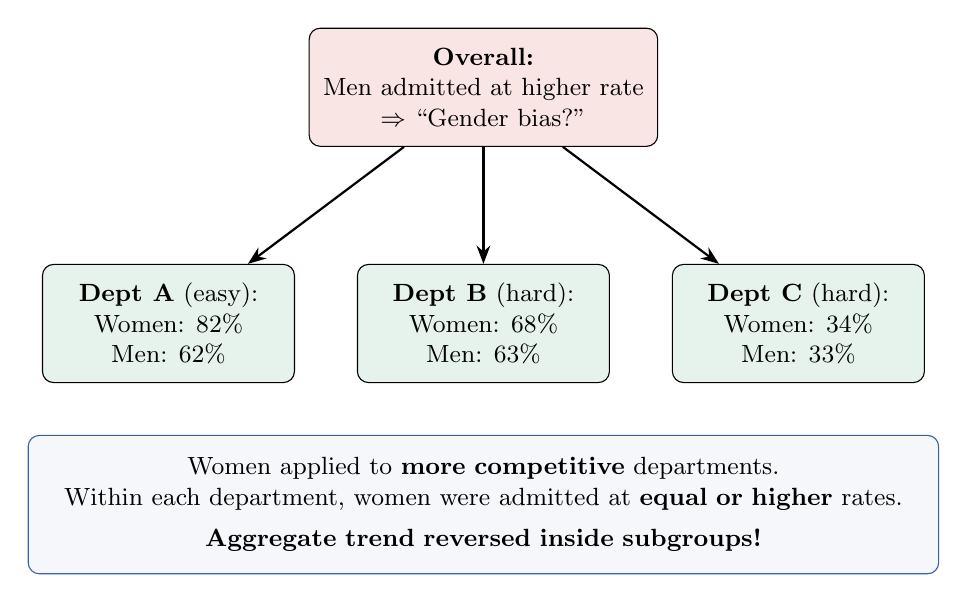
\begin{tikzpicture}[
  deptbox/.style={draw, rounded corners=4pt, minimum width=3.2cm, minimum height=1.5cm, align=center, font=\small, inner sep=5pt}
]
  % Aggregate
  \node[deptbox, fill=sampred!10] (agg) at (0, 2.5) {
    \textbf{Overall:}\\
    Men admitted at higher rate\\
    $\Rightarrow$ ``Gender bias?''
  };

  % Departments
  \node[deptbox, fill=paramgreen!10] (d1) at (-4, -0.5) {
    \textbf{Dept A} (easy):\\
    Women: 82\%\\
    Men: 62\%
  };
  \node[deptbox, fill=paramgreen!10] (d2) at (0, -0.5) {
    \textbf{Dept B} (hard):\\
    Women: 68\%\\
    Men: 63\%
  };
  \node[deptbox, fill=paramgreen!10] (d3) at (4, -0.5) {
    \textbf{Dept C} (hard):\\
    Women: 34\%\\
    Men: 33\%
  };

  \draw[-{Stealth}, thick] (agg) -- (d1);
  \draw[-{Stealth}, thick] (agg) -- (d2);
  \draw[-{Stealth}, thick] (agg) -- (d3);

  % Explanation
  \node[draw=popblue, fill=popblue!5, rounded corners=4pt, text width=11cm, align=center, font=\small, inner sep=8pt] at (0, -2.8) {
    Women applied to \textbf{more competitive} departments.\\
    Within each department, women were admitted at \textbf{equal or higher} rates.\\[4pt]
    \textbf{Aggregate trend reversed inside subgroups!}
  };
\end{tikzpicture}
\end{center}
\end{frame}

% ============================================================
\section{Practical}

\begin{frame}
\frametitle{Practical: Exploratory Data Analysis}
\begin{center}
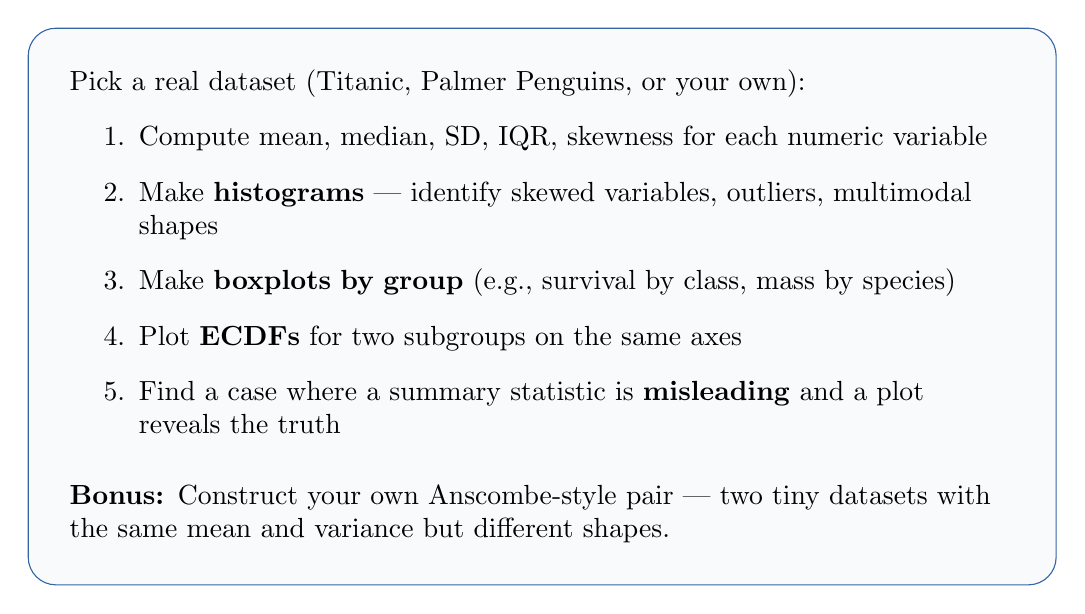
\begin{tikzpicture}
  \node[draw=popblue, fill=popblue!3, rounded corners=10pt, text width=12cm, align=left, inner sep=15pt] {
    Pick a real dataset (Titanic, Palmer Penguins, or your own):
    \begin{enumerate}
      \item Compute mean, median, SD, IQR, skewness for each numeric variable
      \item Make \textbf{histograms} --- identify skewed variables, outliers, multimodal shapes
      \item Make \textbf{boxplots by group} (e.g., survival by class, mass by species)
      \item Plot \textbf{ECDFs} for two subgroups on the same axes
      \item Find a case where a summary statistic is \textbf{misleading} and a plot reveals the truth
    \end{enumerate}
    \vspace{0.2cm}
    \textbf{Bonus:} Construct your own Anscombe-style pair --- two tiny datasets with the same mean and variance but different shapes.
  };
\end{tikzpicture}
\end{center}
\end{frame}

\begin{frame}
\begin{center}
  {\Huge\bfseries\textcolor{popblue}{Questions?}}

  \vspace{1cm}

  {\large Next lecture: Point Estimation --- Maximum Likelihood}
\end{center}
\end{frame}

\end{document}
